% Fig: byte layout of the three encodings of benchmark S2 (field widths
% proportional to bytes; sizes from paper_eval/results/benchmarks.json).
\documentclass[border=2pt]{standalone}
\usepackage{mathptmx}
\usepackage{tikz}
\begin{document}
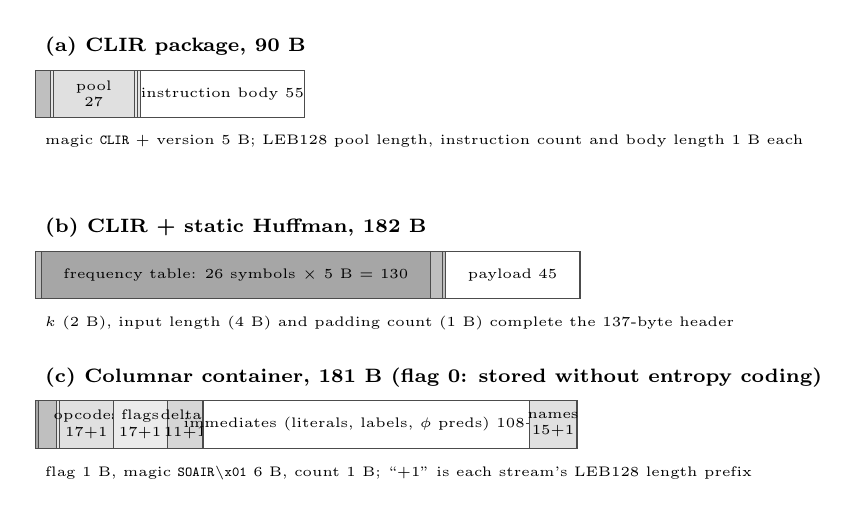
\begin{tikzpicture}[font=\tiny, x=0.38mm, y=1mm]
  % helper: \fld{x0}{width}{row y}{fill}{label}
  \newcommand{\fld}[5]{\draw[fill=#4, draw=black!70] (#1,#3) rectangle ++(#2,-6);
    \node[align=center] at ({#1+#2/2},{#3-3}) {#5};}
  % ---------- (a) CLIR, 90 bytes
  \node[anchor=west, font=\scriptsize\bfseries] at (0,9) {(a) CLIR package, 90 B};
  \fld{0}{5}{6}{black!25}{}
  \fld{5}{1}{6}{black!10}{}
  \fld{6}{27}{6}{black!12}{pool\\27}
  \fld{33}{1}{6}{black!10}{}
  \fld{34}{1}{6}{black!10}{}
  \fld{35}{55}{6}{white}{instruction body 55}
  \node[align=left, anchor=north west] at (0,-1) {magic \texttt{CLIR} + version 5 B; LEB128 pool length, instruction count and body length 1 B each};
  % ---------- (b) Huffman, 182 bytes
  \node[anchor=west, font=\scriptsize\bfseries] at (0,-14) {(b) CLIR + static Huffman, 182 B};
  \fld{0}{2}{-17}{black!25}{}
  \fld{2}{130}{-17}{black!35}{frequency table: 26 symbols $\times$ 5 B = 130}
  \fld{132}{4}{-17}{black!25}{}
  \fld{136}{1}{-17}{black!25}{}
  \fld{137}{45}{-17}{white}{payload 45}
  \node[align=left, anchor=north west] at (0,-24) {$k$ (2 B), input length (4 B) and padding count (1 B) complete the 137-byte header};
  % ---------- (c) Columnar, 181 bytes
  \node[anchor=west, font=\scriptsize\bfseries] at (0,-33) {(c) Columnar container, 181 B (flag 0: stored without entropy coding)};
  \fld{0}{1}{-36}{black!35}{}
  \fld{1}{6}{-36}{black!25}{}
  \fld{7}{1}{-36}{black!10}{}
  \fld{8}{18}{-36}{black!12}{opcodes\\17+1}
  \fld{26}{18}{-36}{black!8}{flags\\17+1}
  \fld{44}{12}{-36}{black!16}{deltas\\11+1}
  \fld{56}{109}{-36}{white}{immediates (literals, labels, $\phi$ preds) 108+1}
  \fld{165}{16}{-36}{black!12}{names\\15+1}
  \node[align=left, anchor=north west] at (0,-43) {flag 1 B, magic \texttt{SOAIR\textbackslash x01} 6 B, count 1 B; ``+1'' is each stream's LEB128 length prefix};
\end{tikzpicture}
\end{document}
